\documentclass[tikz]{standalone}
\usetikzlibrary{shapes.geometric}    % trapezium
\usetikzlibrary{arrows}              % arrow tips
\usepackage{amsmath, amsfonts}
\usepackage{bm}                      % boldsymbol
\usepackage{makecell}                % makecell
\usetikzlibrary{matrix,calc}
\usepackage{color}
\usepackage{xcolor}
\definecolor{mygray}{HTML}{F0F0F0}
\definecolor{myred}{HTML}{CD594A} 
\definecolor{mygreen}{HTML}{829356} 
\definecolor{myblue}{HTML}{3C6478} 
\usepackage{mathtools}
\usetikzlibrary{decorations.pathreplacing}
\begin{document}
    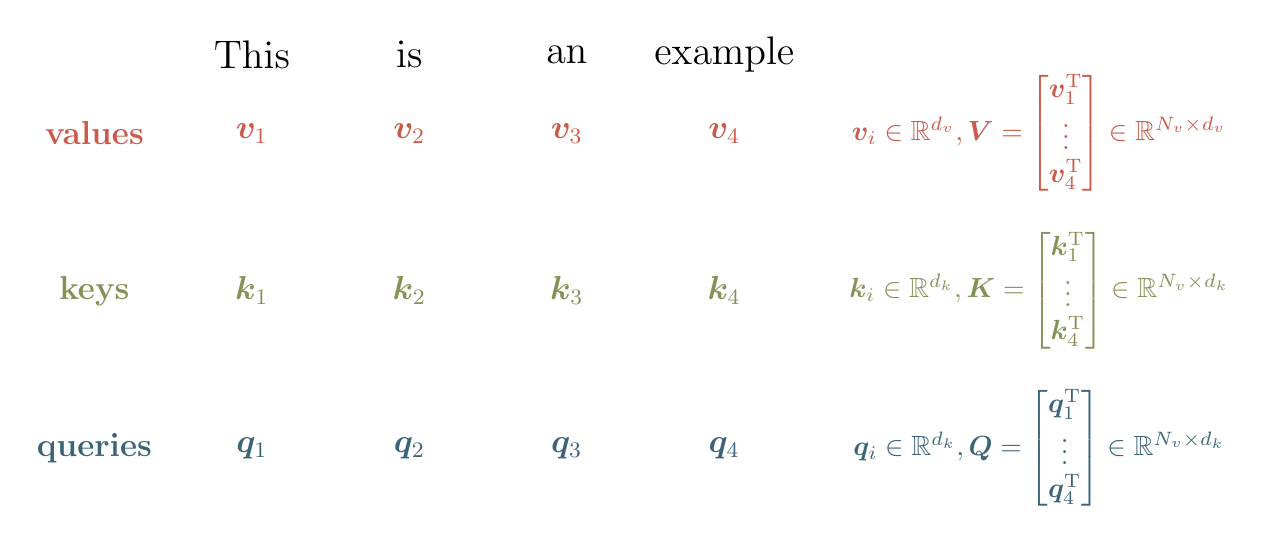
\begin{tikzpicture}[>=latex',thick]

      % TEXT
      \node at (0,0) {\Large{This}};
      \node at (2,0) {\Large{is}};
      \node at (4,0) {\Large{an}};
      \node at (6,0) {\Large{example}};

      % values
      \node at (-2,-1) {\large{\textbf{\textcolor{myred}{values}}}};
      \node at (0, -1) {\large{\textcolor{myred}{$\boldsymbol{v}_1$}}};
      \node at (2, -1) {\large{\textcolor{myred}{$\boldsymbol{v}_2$}}};
      \node at (4, -1) {\large{\textcolor{myred}{$\boldsymbol{v}_3$}}};
      \node at (6, -1) {\large{\textcolor{myred}{$\boldsymbol{v}_4$}}};

      \node at (10, -1)
      {\textcolor{myred}{$
          \boldsymbol{v}_i \in \mathbb{R}^{d_v}, 
          \boldsymbol{V} = \begin{bmatrix}
            \boldsymbol{v}_1^{\text{T}} \\ \vdots \\
            \boldsymbol{v}_4^{\text{T}} \end{bmatrix} \in \mathbb{R}^{N_v \times
            d_v}$}}; 

      % keys 
      \node at (-2,-3) {\large{\textbf{\textcolor{mygreen}{keys}}}};
      \node at (0, -3) {\large{\textcolor{mygreen}{$\boldsymbol{k}_1$}}};
      \node at (2, -3) {\large{\textcolor{mygreen}{$\boldsymbol{k}_2$}}};
      \node at (4, -3) {\large{\textcolor{mygreen}{$\boldsymbol{k}_3$}}};
      \node at (6, -3) {\large{\textcolor{mygreen}{$\boldsymbol{k}_4$}}};

      \node at (10, -3)
      {\textcolor{mygreen}{$
          \boldsymbol{k}_i \in \mathbb{R}^{d_k}, 
          \boldsymbol{K} = \begin{bmatrix}
            \boldsymbol{k}_1^{\text{T}} \\ \vdots \\
            \boldsymbol{k}_4^{\text{T}} \end{bmatrix} \in \mathbb{R}^{N_v \times
            d_k}$}}; 

      % queries
      \node at (-2,-5) {\large{\textbf{\textcolor{myblue}{queries}}}};
      \node at (0, -5) {\large{\textcolor{myblue}{$\boldsymbol{q}_1$}}};
      \node at (2, -5) {\large{\textcolor{myblue}{$\boldsymbol{q}_2$}}};
      \node at (4, -5) {\large{\textcolor{myblue}{$\boldsymbol{q}_3$}}};
      \node at (6, -5) {\large{\textcolor{myblue}{$\boldsymbol{q}_4$}}};

      \node at (10, -5)
      {\textcolor{myblue}{$
          \boldsymbol{q}_i \in \mathbb{R}^{d_k}, 
          \boldsymbol{Q} = \begin{bmatrix}
            \boldsymbol{q}_1^{\text{T}} \\ \vdots \\
            \boldsymbol{q}_4^{\text{T}} \end{bmatrix} \in \mathbb{R}^{N_v \times
            d_k}$}}; 

      % {$\begin{bmatrix} v_{1,1} \\ \vdots \\ v_{1,d_{v}} \end{bmatrix}$};


      % % matrix brackets
      % \draw (-0.5, 0.8) --++(180:3mm)|-(-0.5,-2.2)
      % node [pos=.25, above, rotate=90] {};



      % % row
      % \draw [decorate,decoration={brace,amplitude=10pt,raise=4pt},
      % yshift=12pt] (-0.5,0.8) -- (9.5,0.8) node
      % [black,midway,yshift=0.7cm] {\footnotesize $MR$};
      % \draw [decorate,decoration={brace,amplitude=10pt,raise=4pt},
      % yshift=12pt] (0,0) -- (4,0) node
      % [black,midway,yshift=0.7cm] {\footnotesize $M$ attributes};

      % % time 1
      % \node [circle, draw=black, fill=green!40,
      % label={[xshift=0, yshift=-0.08cm]blue}] at (0, 0) {};
      % \node [circle, draw=black,
      % label={[xshift=0, yshift=-0.08cm]red}] at (1, 0) {};
      % \node [circle, draw=black,
      % label={[xshift=0, yshift=-0.08cm]x=1}] at (2, 0) {};
      % \node [circle, draw=black, fill=green!40,
      % label={[xshift=0, yshift=-0.08cm]x=2}] at (3, 0) {};
      % \node [circle, draw=black,
      % label={[xshift=0, yshift=-0.08cm]x=3}] at (4, 0) {};
      % \node [circle, draw=black,
      % label={[xshift=0, yshift=-0.08cm]blue}] at (5, 0) {};
      % \node [circle, draw=black, fill=green!40,
      % label={[xshift=0, yshift=-0.08cm]red}] at (6, 0) {};
      % \node [circle, draw=black, fill=green!40,
      % label={[xshift=0, yshift=-0.08cm]x=1}] at (7, 0) {};
      % \node [circle, draw=black,
      % label={[xshift=0, yshift=-0.08cm]x=2}] at (8, 0) {};
      % \node [circle, draw=black,
      % label={[xshift=0, yshift=-0.08cm]x=3}] at (9, 0) {};

      % % time 2
      % \node [circle, draw=black, fill=green!40] at (0, -0.6) {};
      % \node [circle, draw=black] at (1, -0.6) {};
      % \node [circle, draw=black] at (2, -0.6) {};
      % \node [circle, draw=black, fill=green!40] at (3, -0.6) {};
      % \node [circle, draw=black] at (4, -0.6) {};
      % \node [circle, draw=black] at (5, -0.6) {};
      % \node [circle, draw=black, fill=green!40] at (6, -0.6) {};
      % \node [circle, draw=black] at (7, -0.6) {};
      % \node [circle, draw=black, fill=green!40] at (8, -0.6) {};
      % \node [circle, draw=black] at (9, -0.6) {};

      % % time 3
      % \node [circle, draw=black, fill=green!40] at (0, -1.2) {};
      % \node [circle, draw=black] at (1, -1.2) {};
      % \node [circle, draw=black] at (2, -1.2) {};
      % \node [circle, draw=black, fill=green!40] at (3, -1.2) {};
      % \node [circle, draw=black] at (4, -1.2) {};
      % \node [circle, draw=black] at (5, -1.2) {};
      % \node [circle, draw=black, fill=green!40] at (6, -1.2) {};
      % \node [circle, draw=black] at (7, -1.2) {};
      % \node [circle, draw=black] at (8, -1.2) {};
      % \node [circle, draw=black, fill=green!40] at (9, -1.2) {};

      % % time 4
      % \node [circle, draw=black, fill=green!40] at (0, -1.8) {};
      % \node [circle, draw=black] at (1, -1.8) {};
      % \node [circle, draw=black] at (2, -1.8) {};
      % \node [circle, draw=black, fill=green!40] at (3, -1.8) {};
      % \node [circle, draw=black] at (4, -1.8) {};
      % \node [circle, draw=black] at (5, -1.8) {};
      % \node [circle, draw=black, fill=green!40] at (6, -1.8) {};
      % \node [circle, draw=black] at (7, -1.8) {};
      % \node [circle, draw=black] at (8, -1.8) {};
      % \node [circle, draw=black, fill=green!40] at (9, -1.8) {};



    \end{tikzpicture}
\end{document}
